\chapter{Introduction}
Given the fact that every human being has the capability of memorizing facts as well as solving problems, any model that tries to mimic the behavior of human brain must constitute a memory component and a problem solving component. The machine learning community represents the problem solving component with an artificial neural network and so far, has been successful in solving tasks such as speech recognition, object classification, image annotation etc. But most of the existing machine learning models lack any interaction with the (potentially very large) long term memory component. That's where the Reasoning, Attention and Memory based machine learning models come into picture.

The models discussed in this thesis comprises of a memory component and a controller, such as an artificial neural network, which takes inputs from external world, stores a representation or encoding of those inputs into the \textbf{memory}, interacts with the memory using a defined mechanism called \textbf{attention} process and produce outputs for the external world with \textbf{reasoning} where the reasoning follows from the graphical visualization of the interaction between controller and memory. Hence, our \textbf{memory} comprises of a set of entities where each entity constitute a representation or encoding of an external input seen by the controller, the \textbf{attention} process is the process or mechanism through which the controller interacts with the memory and the \textbf{reasoning} behind production of an external output follows from the graphical visualization of the interaction between controller and memory. Fig. \ref{fig:gen_arch_ram} shows a general architecture of a RAM based model.

\begin{figure}
\centering
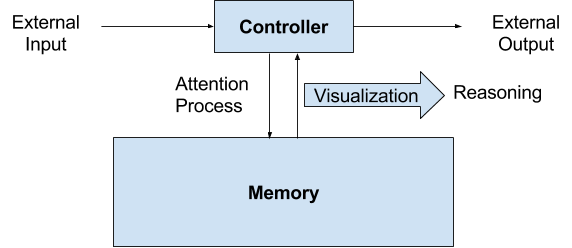
\includegraphics[width=0.75\textwidth]{gen_arch_ram}
\caption{\textbf{General Architecture of a RAM based model}}
\label{fig:gen_arch_ram}
\end{figure}

We now demonstrate why RAM based machine learning models are superior to the existing machine learning models in terms of similarity with the way human beings think. Consider the following comprehension:
\begin{enumerate}
    \itemsep0em 
    \item John went to the kitchen.
    \item John picked up the knife.
    \item John dropped the knife on the floor.
    \item Marry came into the kitchen.
    \item Marry picked up the knife from the floor.
    \item John went to the bathroom.
    \item Marry went to dining room.
\end{enumerate}

Now, try to answer the following query based on the above comprehension: Where is the knife? Your answer must have been ``dining room".

Such question answering tasks have been successfully solved using recurrent neural networks. Recurrent neural networks (RNNs) are a class of artificial neural network architecture that-inspired by the cyclical connectivity of neurons in the brain-uses iterative function loops to store information. Though one might get high accuracy in terms of the correctness of the answer to the query using RNN, but RNN fails to provide an explicit explanation behind the production of a particular answer. On the contrary, RAM based model stores a representation of each sentence of the comprehension as an entity in the memory, searches for the entities in the memory relevant for answering the query and finally computes the answer to the query based on the searched relevant entities.

In this thesis, we focus on applying RAM based models in the domain of sequence to sequence learning where the aim is to find a mapping between a sequence of inputs to a sequence of outputs  and in the domain of building game playing agents where the aim is to find an optimal policy which is a mapping from the state of the agent to a legal action so that, on following the optimal policy, the overall reward or score of the agent gets maximized.

\section{Structure of the Thesis}
Chapter 2 briefly reviews supervised sequence to sequence learning. Chapter 3 reviews reinforcement learning with concepts relevant for understanding chapter 7 of the thesis. Chapter 4 provides background material on artificial neural networks, recurrent neural networks, LSTMs and their training. Chapter 5 and 6 investigates Neural Turing Machine with application in sequence to sequence learning and End to End Memory Networks with application in Q-A tasks, respectively. Chapter 7 proposes a RAM based model for learning the optimal policy for a game playing agent and shows its superiority to existing state of the art in terms of the similarity of the model with the way human beings perceive, reason and act. Chapter 8 provides a brief discussion of the future work.
